\documentclass[tikz,border=8pt]{standalone}
\usepackage{amsmath,amssymb}
\usetikzlibrary{arrows.meta,automata,positioning,quotes}
\begin{document}
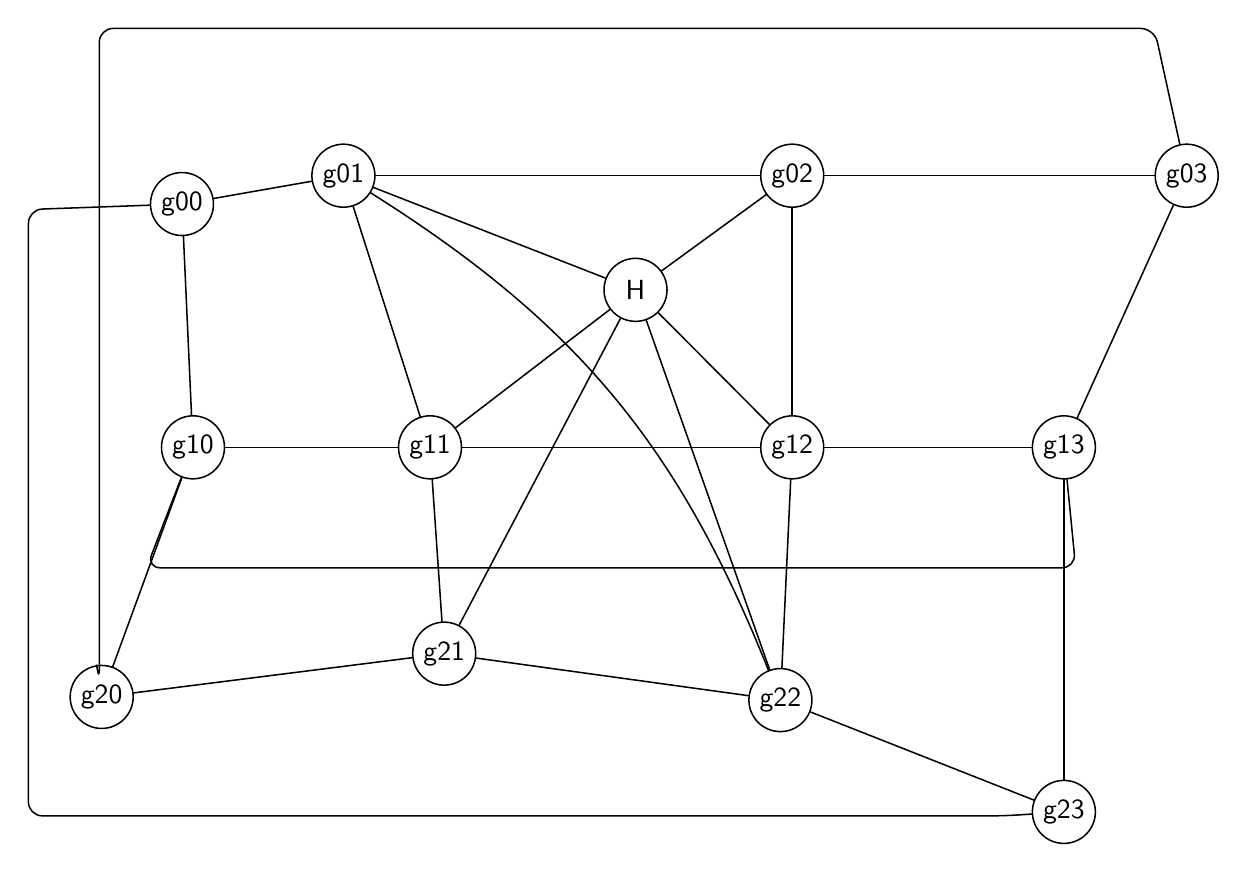
\begin{tikzpicture}[x=1cm,y=1cm]
\tikzset{
  graphnode/.style={circle,draw=black,line width=0.55pt,minimum size=8mm,inner sep=1pt,font=\sffamily},
  graphedge/.style={draw=black,line width=0.55pt,line cap=round,line join=round},
  directed/.style={graphedge,-{Stealth[length=2.4mm,width=2.0mm]}},
  undirected/.style={graphedge}
}
\node[graphnode] (n_g00) at (-0.45,0.07) {g00};
\node[graphnode] (n_g01) at (1.60,0.43) {g01};
\node[graphnode] (n_g02) at (7.30,0.43) {g02};
\node[graphnode] (n_g03) at (12.31,0.43) {g03};
\node[graphnode] (n_g10) at (-0.31,-3.02) {g10};
\node[graphnode] (n_g11) at (2.70,-3.02) {g11};
\node[graphnode] (n_g12) at (7.30,-3.02) {g12};
\node[graphnode] (n_g13) at (10.75,-3.02) {g13};
\node[graphnode] (n_g20) at (-1.47,-6.19) {g20};
\node[graphnode] (n_g21) at (2.88,-5.64) {g21};
\node[graphnode] (n_g22) at (7.15,-6.23) {g22};
\node[graphnode] (n_g23) at (10.75,-7.65) {g23};
\node[graphnode] (n_H) at (5.31,-1.02) {H};
\draw[undirected] (n_g00) -- (n_g01);
\draw[undirected] (n_g01) -- (n_g02);
\draw[undirected] (n_g02) -- (n_g03);
\draw[undirected] (n_g10) -- (n_g11);
\draw[undirected] (n_g11) -- (n_g12);
\draw[undirected] (n_g12) -- (n_g13);
\draw[undirected] (n_g20) -- (n_g21);
\draw[undirected] (n_g21) -- (n_g22);
\draw[undirected] (n_g22) -- (n_g23);
\draw[undirected] (n_g00) -- (n_g10);
\draw[undirected] (n_g10) -- (n_g20);
\draw[undirected] (n_g01) -- (n_g11);
\draw[undirected] (n_g11) -- (n_g21);
\draw[undirected] (n_g02) -- (n_g12);
\draw[undirected] (n_g12) -- (n_g22);
\draw[undirected] (n_g03) -- (n_g13);
\draw[undirected] (n_g13) -- (n_g23);
\draw[undirected] (n_H) -- (n_g01);
\draw[undirected] (n_H) -- (n_g02);
\draw[undirected] (n_H) -- (n_g11);
\draw[undirected] (n_H) -- (n_g12);
\draw[undirected] (n_H) -- (n_g21);
\draw[undirected] (n_H) -- (n_g22);
\draw[undirected,rounded corners=5pt] (n_g00) -- (-2.40,0.00) -- (-2.40,-7.70) -- (10.00,-7.70) -- (n_g23);
\draw[undirected,rounded corners=5pt] (n_g03) -- (11.90,2.30) -- (-1.50,2.30) -- (-1.50,-6.00) -- (n_g20);
\draw[undirected,rounded corners=5pt] (n_g10) -- (-0.90,-4.55) -- (10.90,-4.55) -- (n_g13);
\draw[undirected] (n_g01) to[bend left=18] (n_g22);
\end{tikzpicture}
\end{document}
